% Options for packages loaded elsewhere
\PassOptionsToPackage{unicode}{hyperref}
\PassOptionsToPackage{hyphens}{url}
\PassOptionsToPackage{dvipsnames,svgnames,x11names}{xcolor}
%
\documentclass[
  letterpaper,
  DIV=11,
  numbers=noendperiod]{scrreprt}

\usepackage{amsmath,amssymb}
\usepackage{iftex}
\ifPDFTeX
  \usepackage[T1]{fontenc}
  \usepackage[utf8]{inputenc}
  \usepackage{textcomp} % provide euro and other symbols
\else % if luatex or xetex
  \usepackage{unicode-math}
  \defaultfontfeatures{Scale=MatchLowercase}
  \defaultfontfeatures[\rmfamily]{Ligatures=TeX,Scale=1}
\fi
\usepackage{lmodern}
\ifPDFTeX\else  
    % xetex/luatex font selection
    \setmainfont[]{Noto Sans KR}
\fi
% Use upquote if available, for straight quotes in verbatim environments
\IfFileExists{upquote.sty}{\usepackage{upquote}}{}
\IfFileExists{microtype.sty}{% use microtype if available
  \usepackage[]{microtype}
  \UseMicrotypeSet[protrusion]{basicmath} % disable protrusion for tt fonts
}{}
\makeatletter
\@ifundefined{KOMAClassName}{% if non-KOMA class
  \IfFileExists{parskip.sty}{%
    \usepackage{parskip}
  }{% else
    \setlength{\parindent}{0pt}
    \setlength{\parskip}{6pt plus 2pt minus 1pt}}
}{% if KOMA class
  \KOMAoptions{parskip=half}}
\makeatother
\usepackage{xcolor}
\setlength{\emergencystretch}{3em} % prevent overfull lines
\setcounter{secnumdepth}{5}
% Make \paragraph and \subparagraph free-standing
\makeatletter
\ifx\paragraph\undefined\else
  \let\oldparagraph\paragraph
  \renewcommand{\paragraph}{
    \@ifstar
      \xxxParagraphStar
      \xxxParagraphNoStar
  }
  \newcommand{\xxxParagraphStar}[1]{\oldparagraph*{#1}\mbox{}}
  \newcommand{\xxxParagraphNoStar}[1]{\oldparagraph{#1}\mbox{}}
\fi
\ifx\subparagraph\undefined\else
  \let\oldsubparagraph\subparagraph
  \renewcommand{\subparagraph}{
    \@ifstar
      \xxxSubParagraphStar
      \xxxSubParagraphNoStar
  }
  \newcommand{\xxxSubParagraphStar}[1]{\oldsubparagraph*{#1}\mbox{}}
  \newcommand{\xxxSubParagraphNoStar}[1]{\oldsubparagraph{#1}\mbox{}}
\fi
\makeatother

\usepackage{color}
\usepackage{fancyvrb}
\newcommand{\VerbBar}{|}
\newcommand{\VERB}{\Verb[commandchars=\\\{\}]}
\DefineVerbatimEnvironment{Highlighting}{Verbatim}{commandchars=\\\{\}}
% Add ',fontsize=\small' for more characters per line
\usepackage{framed}
\definecolor{shadecolor}{RGB}{241,243,245}
\newenvironment{Shaded}{\begin{snugshade}}{\end{snugshade}}
\newcommand{\AlertTok}[1]{\textcolor[rgb]{0.68,0.00,0.00}{#1}}
\newcommand{\AnnotationTok}[1]{\textcolor[rgb]{0.37,0.37,0.37}{#1}}
\newcommand{\AttributeTok}[1]{\textcolor[rgb]{0.40,0.45,0.13}{#1}}
\newcommand{\BaseNTok}[1]{\textcolor[rgb]{0.68,0.00,0.00}{#1}}
\newcommand{\BuiltInTok}[1]{\textcolor[rgb]{0.00,0.23,0.31}{#1}}
\newcommand{\CharTok}[1]{\textcolor[rgb]{0.13,0.47,0.30}{#1}}
\newcommand{\CommentTok}[1]{\textcolor[rgb]{0.37,0.37,0.37}{#1}}
\newcommand{\CommentVarTok}[1]{\textcolor[rgb]{0.37,0.37,0.37}{\textit{#1}}}
\newcommand{\ConstantTok}[1]{\textcolor[rgb]{0.56,0.35,0.01}{#1}}
\newcommand{\ControlFlowTok}[1]{\textcolor[rgb]{0.00,0.23,0.31}{\textbf{#1}}}
\newcommand{\DataTypeTok}[1]{\textcolor[rgb]{0.68,0.00,0.00}{#1}}
\newcommand{\DecValTok}[1]{\textcolor[rgb]{0.68,0.00,0.00}{#1}}
\newcommand{\DocumentationTok}[1]{\textcolor[rgb]{0.37,0.37,0.37}{\textit{#1}}}
\newcommand{\ErrorTok}[1]{\textcolor[rgb]{0.68,0.00,0.00}{#1}}
\newcommand{\ExtensionTok}[1]{\textcolor[rgb]{0.00,0.23,0.31}{#1}}
\newcommand{\FloatTok}[1]{\textcolor[rgb]{0.68,0.00,0.00}{#1}}
\newcommand{\FunctionTok}[1]{\textcolor[rgb]{0.28,0.35,0.67}{#1}}
\newcommand{\ImportTok}[1]{\textcolor[rgb]{0.00,0.46,0.62}{#1}}
\newcommand{\InformationTok}[1]{\textcolor[rgb]{0.37,0.37,0.37}{#1}}
\newcommand{\KeywordTok}[1]{\textcolor[rgb]{0.00,0.23,0.31}{\textbf{#1}}}
\newcommand{\NormalTok}[1]{\textcolor[rgb]{0.00,0.23,0.31}{#1}}
\newcommand{\OperatorTok}[1]{\textcolor[rgb]{0.37,0.37,0.37}{#1}}
\newcommand{\OtherTok}[1]{\textcolor[rgb]{0.00,0.23,0.31}{#1}}
\newcommand{\PreprocessorTok}[1]{\textcolor[rgb]{0.68,0.00,0.00}{#1}}
\newcommand{\RegionMarkerTok}[1]{\textcolor[rgb]{0.00,0.23,0.31}{#1}}
\newcommand{\SpecialCharTok}[1]{\textcolor[rgb]{0.37,0.37,0.37}{#1}}
\newcommand{\SpecialStringTok}[1]{\textcolor[rgb]{0.13,0.47,0.30}{#1}}
\newcommand{\StringTok}[1]{\textcolor[rgb]{0.13,0.47,0.30}{#1}}
\newcommand{\VariableTok}[1]{\textcolor[rgb]{0.07,0.07,0.07}{#1}}
\newcommand{\VerbatimStringTok}[1]{\textcolor[rgb]{0.13,0.47,0.30}{#1}}
\newcommand{\WarningTok}[1]{\textcolor[rgb]{0.37,0.37,0.37}{\textit{#1}}}

\providecommand{\tightlist}{%
  \setlength{\itemsep}{0pt}\setlength{\parskip}{0pt}}\usepackage{longtable,booktabs,array}
\usepackage{calc} % for calculating minipage widths
% Correct order of tables after \paragraph or \subparagraph
\usepackage{etoolbox}
\makeatletter
\patchcmd\longtable{\par}{\if@noskipsec\mbox{}\fi\par}{}{}
\makeatother
% Allow footnotes in longtable head/foot
\IfFileExists{footnotehyper.sty}{\usepackage{footnotehyper}}{\usepackage{footnote}}
\makesavenoteenv{longtable}
\usepackage{graphicx}
\makeatletter
\def\maxwidth{\ifdim\Gin@nat@width>\linewidth\linewidth\else\Gin@nat@width\fi}
\def\maxheight{\ifdim\Gin@nat@height>\textheight\textheight\else\Gin@nat@height\fi}
\makeatother
% Scale images if necessary, so that they will not overflow the page
% margins by default, and it is still possible to overwrite the defaults
% using explicit options in \includegraphics[width, height, ...]{}
\setkeys{Gin}{width=\maxwidth,height=\maxheight,keepaspectratio}
% Set default figure placement to htbp
\makeatletter
\def\fps@figure{htbp}
\makeatother
% definitions for citeproc citations
\NewDocumentCommand\citeproctext{}{}
\NewDocumentCommand\citeproc{mm}{%
  \begingroup\def\citeproctext{#2}\cite{#1}\endgroup}
\makeatletter
 % allow citations to break across lines
 \let\@cite@ofmt\@firstofone
 % avoid brackets around text for \cite:
 \def\@biblabel#1{}
 \def\@cite#1#2{{#1\if@tempswa , #2\fi}}
\makeatother
\newlength{\cslhangindent}
\setlength{\cslhangindent}{1.5em}
\newlength{\csllabelwidth}
\setlength{\csllabelwidth}{3em}
\newenvironment{CSLReferences}[2] % #1 hanging-indent, #2 entry-spacing
 {\begin{list}{}{%
  \setlength{\itemindent}{0pt}
  \setlength{\leftmargin}{0pt}
  \setlength{\parsep}{0pt}
  % turn on hanging indent if param 1 is 1
  \ifodd #1
   \setlength{\leftmargin}{\cslhangindent}
   \setlength{\itemindent}{-1\cslhangindent}
  \fi
  % set entry spacing
  \setlength{\itemsep}{#2\baselineskip}}}
 {\end{list}}
\usepackage{calc}
\newcommand{\CSLBlock}[1]{\hfill\break\parbox[t]{\linewidth}{\strut\ignorespaces#1\strut}}
\newcommand{\CSLLeftMargin}[1]{\parbox[t]{\csllabelwidth}{\strut#1\strut}}
\newcommand{\CSLRightInline}[1]{\parbox[t]{\linewidth - \csllabelwidth}{\strut#1\strut}}
\newcommand{\CSLIndent}[1]{\hspace{\cslhangindent}#1}

\usepackage{kotex}
\KOMAoption{captions}{tableheading}
\makeatletter
\@ifpackageloaded{caption}{}{\usepackage{caption}}
\AtBeginDocument{%
\ifdefined\contentsname
  \renewcommand*\contentsname{Table of contents}
\else
  \newcommand\contentsname{Table of contents}
\fi
\ifdefined\listfigurename
  \renewcommand*\listfigurename{List of Figures}
\else
  \newcommand\listfigurename{List of Figures}
\fi
\ifdefined\listtablename
  \renewcommand*\listtablename{List of Tables}
\else
  \newcommand\listtablename{List of Tables}
\fi
\ifdefined\figurename
  \renewcommand*\figurename{Figure}
\else
  \newcommand\figurename{Figure}
\fi
\ifdefined\tablename
  \renewcommand*\tablename{Table}
\else
  \newcommand\tablename{Table}
\fi
}
\@ifpackageloaded{float}{}{\usepackage{float}}
\floatstyle{ruled}
\@ifundefined{c@chapter}{\newfloat{codelisting}{h}{lop}}{\newfloat{codelisting}{h}{lop}[chapter]}
\floatname{codelisting}{Listing}
\newcommand*\listoflistings{\listof{codelisting}{List of Listings}}
\usepackage{amsthm}
\theoremstyle{definition}
\newtheorem{example}{Example}[chapter]
\theoremstyle{definition}
\newtheorem{definition}{Definition}[chapter]
\theoremstyle{remark}
\AtBeginDocument{\renewcommand*{\proofname}{Proof}}
\newtheorem*{remark}{Remark}
\newtheorem*{solution}{Solution}
\newtheorem{refremark}{Remark}[chapter]
\newtheorem{refsolution}{Solution}[chapter]
\makeatother
\makeatletter
\makeatother
\makeatletter
\@ifpackageloaded{caption}{}{\usepackage{caption}}
\@ifpackageloaded{subcaption}{}{\usepackage{subcaption}}
\makeatother
\makeatletter
\@ifpackageloaded{algorithm}{}{\usepackage{algorithm}}
\makeatother
\makeatletter
\@ifpackageloaded{algpseudocode}{}{\usepackage{algpseudocode}}
\makeatother
\makeatletter
\@ifpackageloaded{fontspec}{}{\usepackage{fontspec}}
\makeatother
\makeatletter
\@ifpackageloaded{draftwatermark}{}{\usepackage{draftwatermark}}
\makeatother
\makeatletter
\@ifpackageloaded{xcolor}{}{\usepackage{xcolor}}
\makeatother
\makeatletter
\@ifpackageloaded{forloop}{}{\usepackage{forloop}}
\makeatother
    \definecolor{watermark}{HTML}{000000}
    
    \newcounter{watermarkrow}
    \newcounter{watermarkcol}

    \DraftwatermarkOptions{
      text={
        \begin{tabular}{c}
          \forloop{watermarkrow}{0}{\value{watermarkrow} < 50}{
            \forloop{watermarkcol}{0}{\value{watermarkcol} < 10}{
              { Seoncheol\ Park}\hspace{4.000000em}
            }
            \\[4.000000em]
          }
        \end{tabular}
      },
      fontsize=1.000000em,
      angle=15.000000,
      color=watermark!10
    }
    
\ifLuaTeX
  \usepackage{selnolig}  % disable illegal ligatures
\fi
\usepackage{bookmark}

\IfFileExists{xurl.sty}{\usepackage{xurl}}{} % add URL line breaks if available
\urlstyle{same} % disable monospaced font for URLs
\hypersetup{
  pdftitle={Computational Satistics},
  pdfauthor={Seoncheol Park},
  colorlinks=true,
  linkcolor={blue},
  filecolor={Maroon},
  citecolor={Blue},
  urlcolor={Blue},
  pdfcreator={LaTeX via pandoc}}

\title{Computational Satistics}
\author{Seoncheol Park}
\date{2024-06-01}

\begin{document}
\maketitle

\renewcommand{\Return}{\State \textbf{return}~}
\newcommand{\Print}{\State \textbf{print}~}
\newcommand{\Break}{\State \textbf{break}}
\newcommand{\Continue}{\State \textbf{continue}}
\newcommand{\True}{\textbf{true}}
\newcommand{\False}{\textbf{false}}
\renewcommand{\And}{\textbf{and}~}
\newcommand{\Or}{\textbf{or}~}
\renewcommand{\Not}{\textbf{not}~}
\newcommand{\To}{\textbf{to}~}
\newcommand{\DownTo}{\textbf{downto}~}

\floatname{algorithm}{Algorithm}

\renewcommand*\contentsname{Table of contents}
{
\hypersetup{linkcolor=}
\setcounter{tocdepth}{2}
\tableofcontents
}
\chapter*{Preface}\label{preface}
\addcontentsline{toc}{chapter}{Preface}

\markboth{Preface}{Preface}

This is a Quarto book.

To learn more about Quarto books visit
\url{https://quarto.org/docs/books}.

\begin{Shaded}
\begin{Highlighting}[]
\DecValTok{1} \SpecialCharTok{+} \DecValTok{1}
\end{Highlighting}
\end{Shaded}

\begin{verbatim}
[1] 2
\end{verbatim}

\part{Intro}

\chapter{Introduction}\label{introduction}

This is a book created from markdown and executable code.

See Knuth (1984) for additional discussion of literate programming.

\begin{Shaded}
\begin{Highlighting}[]
\DecValTok{1} \SpecialCharTok{+} \DecValTok{1}
\end{Highlighting}
\end{Shaded}

\begin{verbatim}
[1] 2
\end{verbatim}

\part{Optimization Methods}

\chapter{최적화 방법}\label{uxcd5cuxc801uxd654-uxbc29uxbc95}

\section{Optimization}\label{optimization}

통계에서 최적화를 해야 하는 상황

\begin{itemize}
\tightlist
\item
  Maximum likelihood \(\max_{\theta} L(\theta | \pmb{y})\)
\end{itemize}

\section{Maximum Likelihood Theory}\label{maximum-likelihood-theory}

\begin{itemize}
\item
  For independent data: \textbf{likelihood function} \[
  L(\theta) = \prod_{i=1}^n f(\pmb{x}_i | \theta)
  \]
\item
  \textbf{Log-likelihood function} \[
  \ell (\theta) = \sum_{i=1}^n \log (f(\pmb{x}_i ; \theta))
  \]
\item
  Maximum likelihood estimate:
  \(\hat{\theta}_{\text{ML}}=\text{argmax}_{\theta} L(\theta)\)
\item
  For smooth likelihoods, necessary requirement:
\end{itemize}

\begin{align*}
\pmb{s}(\pmb{\theta}) &\equiv \ell ' (\pmb{\theta}), \quad{} |\pmb{\theta}| \text{ equations, called score vector}\\
\pmb{J}(\pmb{\theta}) &\equiv -\ell '' (\pmb{\theta}), \quad{}\text{ positive (definite), called observed Fisher information}
\end{align*}

\begin{itemize}
\tightlist
\item
  Theory:

  \begin{itemize}
  \tightlist
  \item
    \(E[\pmb{s}(\pmb{\theta})] = 0\)
  \item
    \(\pmb{I}(\pmb{\theta}) \equiv - E[\ell '' (\pmb{\theta})] = E[\pmb{J}(\pmb{\theta})]= \text{Var}[\pmb{s}(\pmb{\theta})], \quad{} \text{expected Fisher information}\)
  \item
    For large \(n\) (and some regularity assumptions) \[
    \hat{\pmb{\theta}}_{\text{Ml}} \approx \mathcal{N}(\pmb{\theta}, \pmb{I}^{-1}(\hat{\pmb{\theta}}_{\text{ML}})) \approx \mathcal{N}(\pmb{\theta}, \pmb{J}^{-1}(\hat{\pmb{\theta}}_{\text{ML}}))
    \]
  \end{itemize}
\end{itemize}

\section{Newton의 방법}\label{newtonuxc758-uxbc29uxbc95}

\textbf{Q}. 뉴턴법은 언제 쓰는가?

\begin{itemize}
\item
  \(f(x)=0\)의 해를 근사적으로 구할 때
\item
  \(g(x)=h(x)\)인 \(x\)를 근사적으로 구할 때
\item
  \(f(x)\)의 최소값 또는 최대값을 구할 때
\end{itemize}

\textbf{Q}. 뉴턴법의 한계

\begin{itemize}
\item
  해가 여러개 일 경우
\item
  수렴속도가 초깃값에 따라 달라짐
\end{itemize}

\textbf{Q}. 통계에서의 뉴턴법? ML estimation

1차원에서의 ML 추정을 생각해보자. \[
\text{argmax}_{\theta} L(\theta | \pmb{y}) = \text{argmax}_{\pmb{\theta}}\underbrace{\log L(\theta | \pmb{y})}_{\ell (\theta | \pmb{y})}
\]

이것을 \(\theta^{*}\) 근처에서 테일러 근사로 전개해보자.

\begin{align*}
\ell (\theta) &\approx \ell (\theta^{*}) + (\theta - \theta^{*}) \ell ' (\theta^{*}) + \frac{1}{2}(\theta - \theta^{*})^2 \ell '' (\theta^{*})\\
&= \ell (\theta^{*}) + (\theta - \theta^{*}) s (\theta^{*}) - \frac{1}{2}(\theta - \theta^{*})^2 J (\theta^{*})
\end{align*}

즉 score 함수는 \(s(\theta) = \ell ' (\theta)\), observed information은
\(J(\theta) = - \ell '' (\theta)\)이다.

\begin{itemize}
\tightlist
\item
  Solving the maximum of the approximation \[
  \theta = \theta^{*} + \frac{s(\theta^{*})}{J(\theta^{*})} = \theta^{*} - \frac{\ell ' (\theta^{*})}{\ell '' (\theta^{*})}
  \]
\end{itemize}

\subsection{Stoping criteria}\label{stoping-criteria}

\begin{itemize}
\tightlist
\item
  반복법에서는 어느 시점에 어떤 기준을 가지고 멈춰야 할지를 정하는 것이
  중요하다.
\end{itemize}

\begin{enumerate}
\def\labelenumi{\arabic{enumi}.}
\item
  Absolute convergence: 이는 \(x\)가 클 경우에 시간이 오래 걸릴 수 있다.
  \[|x^{(t+1)} -x^{(t)}| < \varepsilon \text{ or }\| \pmb{x}^{(t+1)} - \pmb{x}^{(t)} \| < \varepsilon\]
\item
  Relative convergence: 이는 \(|x^{(t)}|\)가 작을 경우에 불안정할 수
  있다. \[
  \frac{|x^{(t+1)}- x^{(t)}|}{|x^{(t)}|} < \varepsilon \text{ or }\frac{\|x^{(t+1)}- x^{(t)}\|}{\|x^{(t)}\|} < \varepsilon
  \]
\item
  After \(N\) iterations (additional criteria)
\end{enumerate}

\subsection{Log likelihood의 score와 observed
information}\label{log-likelihooduxc758-scoreuxc640-observed-information}

\begin{itemize}
\item
  Likelihood fct (\(\sigma\) is known) \[
  L(\mu) = \prod_{i=1}^n \frac{1}{\sqrt{2\pi\sigma^2}} \exp \Big\{-\frac{1}{2}\Big( \frac{x_i- \mu}{\sigma} \Big)^2 \Big\}
  \]
\item
  Log-likelihood \[
  \ell(\mu) = \sum_{i=1}^n -\frac{1}{2}\log 2\pi - \frac{1}{2}\log \sigma^2 - \frac{1}{2}\Big( \frac{x_i -\mu}{\sigma} \Big)^2
  \]
\item
  Score fct \[
  s(\mu) = \ell ' (\mu) = \sum_{i=1}^n -0 - 0 - \frac{x_i - \mu}{\sigma^2} = \frac{1}{\sigma^2} \sum_{i=1}^n  (x_i - \mu)
  \]
\item
  Information \[
  J(\mu) = -\ell '' (\mu) = - s' (\mu) = - \frac{1}{\sigma^2}\sum_{i=1}^n (-1) = \frac{n}{\sigma^2}
  \]
\end{itemize}

\subsection{Multidimensional
extension}\label{multidimensional-extension}

\begin{itemize}
\item
  Consider log likelihood: \[
  \text{argmax}_{\pmb{\theta}} \ell (\pmb{\theta}) = \text{argmax}_{\pmb{\theta}} L(\pmb{\theta}|\pmb{y})= \text{argmax}_{\pmb{\theta}} \log( L(\pmb{\theta}|\pmb{y}) )
  \]
\item
  그러면 다차원에서 테일러 근사는 다음과 같다.
\end{itemize}

\begin{align*}
\ell (\pmb{\theta}) &\approx \ell (\pmb{\theta}^{*}) + (\pmb{\theta} - \pmb{\theta}^{*})^T \ell ' (\pmb{\theta}^{*}) + \frac{1}{2} (\pmb{\theta} - \pmb{\theta}^{*})^T \pmb{H}(\pmb{\theta}^{*})(\pmb{\theta}-\pmb{\theta}^{*})\\
&\approx \ell (\pmb{\theta}^{*}) + (\pmb{\theta} - \pmb{\theta}^{*})^T \pmb{s} (\pmb{\theta}^{*}) - \frac{1}{2} (\pmb{\theta} - \pmb{\theta}^{*})^T \pmb{J}(\pmb{\theta}^{*})(\pmb{\theta}-\pmb{\theta}^{*})
\end{align*}

\begin{itemize}
\item
  Score function: \[
  \pmb{s} (\pmb{\theta}) = \nabla \ell (\pmb{\theta}) = \frac{\partial}{\partial \pmb{\theta}} \ell (\pmb{\theta})
  \]
\item
  Observed information: \[
  \pmb{J} (\pmb{\theta}) = -\nabla^2 \ell (\pmb{\theta}) = \frac{\partial^2}{\partial \pmb{\theta}^2}\ell (\pmb{\theta})
  \]
\item
  여기서는 반복법을 이용해 다음의 근사를 풀어 최대화한다. \[
  \pmb{\theta} = \pmb{\theta}^{*} + \pmb{J}(\pmb{\theta}^{*})^{-1}\pmb{s}(\pmb{\theta}^{*}) = \pmb{\theta}^{*} - \pmb{H}(\pmb{\theta}^{*})^{-1}\nabla \ell (\pmb{\theta}^{*})
  \]
\end{itemize}

\subsection{\texorpdfstring{\(\mathbb{R}^p\)에서의 log likelihood의
score와 observed
information}{\textbackslash mathbb\{R\}\^{}p에서의 log likelihood의 score와 observed information}}\label{mathbbrpuxc5d0uxc11cuxc758-log-likelihooduxc758-scoreuxc640-observed-information}

\begin{itemize}
\item
  Likelihood: \(\Sigma\)가 알려져 있다고 할 때 \[
  L(\mu) = \prod_{i=1}^n \frac{1}{\sqrt{(2\pi)^p |\Sigma|}}\exp \Big\{ - \frac{1}{2}(x_i - \mu)^T \Sigma^{-1}(x_i - \mu) \Big\}
  \]
\item
  Log-likelihood \[
  \ell (\mu) = \sum_{i=1}^n -\frac{p}{2}\log 2\pi - \frac{1}{2}\log |\Sigma | - \frac{1}{2} (x_i - \mu)^T \Sigma^{-1}(x_i - \mu)
  \]
\item
  Score function \[
  s(\mu) = \nabla \ell (\mu) = \sum_{i=1}^n \Sigma^{-1} (x_i - \mu) = \Sigma^{-1}\sum_{i=1}^n (x_i - \mu)
  \]
\item
  Information \[
  J(\mu) = - \nabla^2 \ell (\mu) = - \sum_{i=1}^n -\Sigma^{-1} = n \Sigma^{-1} = \Big( \frac{1}{n}\Sigma \Big)^{-1}
  \]
\end{itemize}

\section{Fisher scoring}\label{fisher-scoring}

\begin{itemize}
\item
  뉴턴의 방법은 \(\ell'' (\theta) <0\)이거나 \(J(\theta) >0\)이라는
  조건을 필요로 한다. 다변량에서는 \(\pmb{J}(\pmb{\theta})\)가 positive
  definite여야 한다.
\item
  \(\pmb{J}(\pmb{\theta})\)는 stochastic (depend on data)
\item
  \(\pmb{I}(\pmb{\theta}) = E[ \pmb{J}(\pmb{\theta})]\):
  \textbf{expected information matrix}
\item
  이때 \(\pmb{I}(\pmb{\theta}) = \text{Var}[\pmb{s}(\pmb{\theta})]\)가
  항상 positive (semi-)definite임을 보일 수 있다.
\end{itemize}

\textbf{Fisher scoring algorithm}은 다음과 같다. \[
\pmb{\theta}^{(t+1)} = \pmb{\theta}^{(t)} + [\pmb{I}(\pmb{\theta}^{(t)})]^{-1}\pmb{s}(\pmb{\theta}^{(t)})
\] 이렇게 하면 계산이 좀 더 쉬워지고 뉴턴의 방법에 비해 좀 더 안정적으로
된다고 한다.

\begin{example}[\(p\)차원에서 정규분포를 따르는 자료의
\(\pmb{I}(\pmb{\theta})\)]\protect\hypertarget{exm-Aitken}{}\label{exm-Aitken}

\(\mathbb{R}^p\)에서 \(I(\mu) = E(J(\mu)) = \text{Var}(s(\mu))\)임을
보일 수 있다.

\begin{itemize}
\item
  \(s(\mu) = \Sigma^{-1} \sum_{i=1}^n (x_i - \mu)\)
\item
  \(J(\mu) = \Big( \frac{1}{n}\Sigma \Big)^{-1}\)
\item
  \(E(J(\mu)) = E\Big( (\frac{1}{n}\Sigma)^{-1} \Big)= (\frac{1}{n|\Sigma)^{-1}\)
\item
  \(s(\mu)\)의 분산
\end{itemize}

\begin{align*}
\text{Var}(s(\mu)) &= \text{Var} \Big( \Sigma^{-1} \sum_{i=1}^n (x_i - \mu)\Big)\\
&= \sum_{i=1}^n \Sigma^{-1}\text{Var}(x_i - \mu)\Sigma^{-1} \quad{} (\because \text{independence})\\
&= \sum_{i=1}^n \Sigma^{-1}\Sigma \Sigma^{-1} = n \Sigma^{-1}\\
&= \Big( \frac{1}{n}\Sigma \Big)^{-1}
\end{align*}

\end{example}

\section{Gauss-Newton method}\label{gauss-newton-method}

\textbf{Q}. 가우스-뉴턴법: 뉴턴법을 연립방정식 형태로 확장시킨 것(??)

\begin{itemize}
\tightlist
\item
  다음과 같은 모형을 생각해보자. \[
  Y_i = f(\pmb{z}_i ; \pmb{\theta}) + \varepsilon_i
  \] 그리고
  \(g(\pmb{\theta}) = -\sum_{i=1}^n (y_i - f(\pmb{z}_i; \pmb{\theta}))^2\)을
  최대화하고자 한다.
\end{itemize}

\begin{enumerate}
\def\labelenumi{\arabic{enumi}.}
\item
  뉴턴의 방법은 \(g(\pmb{\theta})\)를 근사하는 방법이다.
\item
  가우스-뉴턴의 방법은 \(f(\pmb{z}_i;\pmb{\theta})\)를 근사하는
  방법이다. \[
  \tilde{f}(\pmb{z}_i ; \pmb{\theta}; \pmb{\theta}^{(t)}) \approx f(\pmb{z}_i; \pmb{\theta}^{(t)}) + (\pmb{\theta} - \pmb{\theta}^{(t)})\nabla_{\pmb{\theta}} f(\pmb{z}_i, \pmb{\theta}^{(t)})
  \]
\end{enumerate}

\begin{itemize}
\tightlist
\item
  Gauss-Newton step은 다음을 최대화하는 것이다:
\end{itemize}

\begin{align*}
\tilde{g}(\pmb{\theta}) &= - \sum_{i=1}^n (y_i - \tilde{f}(\pmb{z}_i ; \pmb{\theta}; \pmb{\theta}^{(t)}))^2\\
&= -\sum_{i=1}^n [y_i - f(\pmb{z}_i; \pmb{\theta}^{(t)})+ (\pmb{\theta}-\pmb{\theta}^{(t)})^T\nabla_{\pmb{\theta}}f(\pmb{z}_i, \pmb{\theta}^{(t)})]^2
\end{align*}

\begin{itemize}
\item
  이것의 해(solution)는 다음과 같다: \[
  \pmb{\theta}^{(t+1)} = \pmb{\theta}^{(t)}+ [(\pmb{A}^{(t)})^T\pmb{A}^{(t)} ]^{-1}(\pmb{A}^{(t)})^T[\pmb{y} - \pmb{f}(\pmb{z}; \pmb{\theta}^{(t)})]
  \] 이때 \[
  \pmb{f}(\pmb{z}; \pmb{\theta}) = \begin{bmatrix}
  f(\pmb{z}_1;\pmb{\theta})\\
  \vdots\\
  f(\pmb{z}_n;\pmb{\theta})
  \end{bmatrix}, \quad{}
  \pmb{A}^{(t)}_{n\times p} = \begin{bmatrix}
  \nabla_{\theta} f(\pmb{z}_1, \theta)\\
  \vdots\\
  \nabla_{\theta} f(\pmb{z}_n, \theta)
  \end{bmatrix}
  \]
\item
  장점: first derivatives만 있어도 된다.
\end{itemize}

\subsection{회귀분석에서의
가우스-뉴턴법}\label{uxd68cuxadc0uxbd84uxc11duxc5d0uxc11cuxc758-uxac00uxc6b0uxc2a4-uxb274uxd134uxbc95}

\begin{itemize}
\tightlist
\item
  회귀분석: 다음을 푸는 것 \[
  \min_{\beta} \sum_{i=1}^n (y_i - \beta^T x_i)^2
  \]
\end{itemize}

\(\pmb{X} = \begin{bmatrix} x_1 \\ \vdots \\ x_n \end{bmatrix}\)이라고
할 때 최소제곱법으로 구하면 다음과 같다.

\begin{align*}
&\min_{\pmb{\beta}}(\pmb{y} - \pmb{X}\pmb{\beta})^T(\pmb{y} - \pmb{X}\pmb{\beta})\\
&\frac{\partial}{\partial\pmb{\beta}} 2\pmb{X}^T(\pmb{y}-\pmb{X\beta})=0\\
&\pmb{\beta} = (\pmb{X}^T\pmb{X})^{-1}\pmb{X}^T\pmb{y}
\end{align*}

\begin{itemize}
\tightlist
\item
  이것을 근사 방법으로 풀면 다음과 같다.
\end{itemize}

\begin{align*}
&\min_{\pmb{\beta}}\sum_{i=1}^n (y_i - f(z_i, \theta))^2\\
&\min_{\pmb{\beta}}\sum_{i=1}^n (y_i - f(z_i, \theta_k)- (\theta-\theta_k)^T\nabla f(z_i, \theta_k))^2\\
\theta_{k+1} &= \theta_k + \Big( \pmb{A}^{(k)^T}\pmb{A}^{(k)}  \Big)^{-1}\pmb{A}^{(k)^T}(\pmb{y}-\pmb{f}(\pmb{z};\pmb{\theta}))
\end{align*}

이때 \[
\pmb{f}(\pmb{z};\pmb{\theta}) = 
\begin{bmatrix}
f(\pmb{z}_1; \pmb{\theta})\\
\vdots\\
f(\pmb{z}_n; \pmb{\theta})
\end{bmatrix}, \quad{}
\pmb{A}^{(k)}= 
\begin{bmatrix}
\nabla_{\pmb{\theta}}f(\pmb{z}_1,\theta_k)\\
\vdots\\
\nabla_{\pmb{\theta}}f(\pmb{z}_n,\theta_k)
\end{bmatrix}
\]

종합적으로 정리하면 뉴턴류의 방법은 미분계수가 필요하다.

\section{Other optimization methods}\label{other-optimization-methods}

\begin{itemize}
\item
  \textbf{Secant methods}: Replace \(J(\theta) = -\ell '' (\theta)\) by
  finite difference approximation
\item
  \textbf{Fixed-point} methods (\(\max_x g(x)\))

  \begin{itemize}
  \tightlist
  \item
    Find function \(G(x)\) such that
    \(G(x) = x \Longleftrightarrow g'(x) = 0\)
  \item
    Use updating scheme \(x^{(t+1)} = G(x^{(t)})\)
  \item
    Obvious choice:
    \(G(x) = \alpha g' (x) + x \Longrightarrow x^{(t+1)} = x^{(t)} + \alpha g'(x^{(t)})\)
  \item
    Requirements for convergence: (1)
    \(x \in [a,b] \Longrightarrow G(x) \in [a,b]\), (2)
    \(|G(x_1) - G(x_2) | \leq \lambda |x_1 - x_2|\) for all
    \(x_1, x_2 \in [a,b]\) for some \(\lambda \in (0,1)\)
  \end{itemize}
\end{itemize}

\section{Fixed Point}\label{fixed-point}

\begin{itemize}
\item
  다음의 예를 보자. \[
  \text{argmax}_{x} g(x) = x\log (x) - x + 0.5x^2, \quad{} g'(x) = \log (x) + x
  \]
\item
  Possible choices of \(G\): \[
  \begin{align*}
  G_1 (x) &= g'(x) + x = \log (x) + 2x\\
  G_2 (x) &= - \log (x)\\
  G_3 (x) &= \exp (-x)\\
  G_4 (x) &= (x+\exp(-x))/2
  \end{align*}
  \]
\end{itemize}

\begin{verbatim}
Warning in log(x[2]): NaNs produced
\end{verbatim}

\begin{figure}[H]

{\centering \includegraphics[width=0.7\textwidth,height=\textheight]{optim_files/figure-pdf/unnamed-chunk-1-1.pdf}

}

\caption{Figure: Forward stepwise regression output.}

\end{figure}%

\begin{verbatim}
          [,1]      [,2]         [,3]       [,4]
  1.000000e+01 10.000000 1.000000e+01 10.0000000
x 2.230259e+01 -2.302585 4.539993e-05  5.0000227
x 4.770987e+01       NaN 9.999546e-01  2.5033802
x 9.928488e+01       NaN 3.678961e-01  1.2925941
x 2.031678e+02       NaN 6.921891e-01  0.7835759
x 4.116496e+02       NaN 5.004793e-01  0.6201728
x 8.293193e+02       NaN 6.062400e-01  0.5790121
x 1.665359e+03       NaN 5.453977e-01  0.5697319
x 3.338136e+03       NaN 5.796112e-01  0.5677045
x 6.684385e+03       NaN 5.601161e-01  0.5672648
x 1.337758e+04       NaN 5.711428e-01  0.5671696
x 2.676466e+04       NaN 5.648795e-01  0.5671490
x 5.353951e+04       NaN 5.684286e-01  0.5671445
x 1.070899e+05       NaN 5.664148e-01  0.5671436
x 2.141914e+05       NaN 5.675566e-01  0.5671433
x 4.283951e+05       NaN 5.669089e-01  0.5671433
x 8.568031e+05       NaN 5.672762e-01  0.5671433
x 1.713620e+06       NaN 5.670679e-01  0.5671433
x 3.427254e+06       NaN 5.671860e-01  0.5671433
x 6.854523e+06       NaN 5.671190e-01  0.5671433
x 1.370906e+07       NaN 5.671570e-01  0.5671433
\end{verbatim}

\chapter{Gradient Descent}\label{gradient-descent}

\section{Basic Setting}\label{basic-setting}

\begin{itemize}
\item
  Goal: minimize some \(F(\theta)\) w.r.t. \(\theta\)
\item
  \textbf{Empirical risk}: \[
  F(\theta) = \frac{1}{n}\sum_{i=1}^n f_i (\theta) + J(\theta)
  \]
\item
  Options for \(f_i (\theta)\): \[
  f_i (\theta) = 
  \begin{cases}
  (\hat{y}_i - y_i)^, & \text{Least squares}\\
  I(\hat{y}_i \neq y_i), & \text{Classification error}\\
  -\log f(y_i; \theta), & \text{Log-likelihood}
  \end{cases}
  \]
\item
  Alternative: \textbf{Expected risk} \[
  F(\theta) = E[f(\theta; \pmb{\varepsilon})], \quad{}\pmb{\varepsilon} \text{ is some random vector}
  \]
\item
  \(F(\cdot)\) is nice and smooth, a necessary requirement is \[
  \pmb{g}(\pmb{\theta}^{*}) = \frac{\partial}{\partial \pmb{\theta}}F(\pmb{\theta})|_{\pmb{\theta}=\pmb{\theta}^{*}} = \pmb{0}
  \]
\end{itemize}

\section{Ordinary Gradient Descent}\label{ordinary-gradient-descent}

\begin{itemize}
\item
  Ordinary gradient descent: \[
  \pmb{\theta}^{t+1} = \pmb{\theta}^{t} - \pmb{M}_t^{-1}\pmb{g}(\pmb{\theta}^t), \quad{} \pmb{M}_t \text{ is p.d.}
  \]
\item
  Problem: Gradient might be difficult to compute
\end{itemize}

\section{Stochastic Gradient Descent}\label{stochastic-gradient-descent}

\begin{itemize}
\item
  The \textbf{stochastic gradient} algorithm replaces the gradient by an
  \textbf{estimate} instead: \[
  \pmb{\theta}^{t+1} = \pmb{\theta}^t -\alpha_t \pmb{M}_t^{-1}\pmb{Z}(\pmb{\theta}^{t};\pmb{\phi}^t), \quad{} \pmb{Z}(\pmb{\theta}^T; \pmb{\phi}^t) \approx \pmb{g} (\pmb{\theta}^t)
  \]
\item
  A class of possibilities are given by \[
  \pmb{Z}(\pmb{\theta}^{t}; \pmb{\phi}^t) = \frac{1}{n_t} \sum_{i \in \mathcal{S}_t} \nabla f_i (\pmb{\theta}^t), \quad{} \mathcal{S}_t \subset \{ 1, \ldots, n\}, \quad{} n_t = |\mathcal{S}_t|
  \]
\end{itemize}

\begin{algorithm}[htb!]
\caption{Stochastic gradient descent}
\label{alg-sgd}
\begin{algorithmic}[1]
\Procedure{SGD}{$\pmb{Z},\pmb{\theta}, \pmb{\phi}$}
  \For{$t = 1$ \To $\cdots$}
    \State Simulate the stochastic gradient $\pmb{Z}(\pmb{\theta}^t; \pmb{\phi}^t)$
    \State Choose a step size $\alpha$'
    \State Update the new value by $\pmb{\theta}^{t+1} \leftarrow \pmb{\theta}^{t}  - \alpha_t \pmb{M}_t^{-1}\pmb{Z} (\pmb{\theta}^t; \pmb{\phi}^t)$
  \EndFor
\EndProcedure
\end{algorithmic}
\end{algorithm}

::: \{\#exm-logistic sgd\}

\section{Logistic Regression}\label{logistic-regression}

Logistic regression with \(n\) is large:

\begin{align*}
Y_i &\sim \text{Binomial}(1, p(x_i)), \quad{} i=1, \ldots, n\\
p(x_i) &= \frac{\exp (\theta_0 + \theta_1 \pmb{x})}{1+\exp (\theta_0 + \theta_1 \pmb{x})}
\end{align*}

Want to minimize

\begin{align*}
F(\pmb{\theta}) &= -\sum_{i=1}^n [y_i \log (p_i) + (1-y_i) \log (1-p_i)]\\
&= -\sum_{i=1}^n [y_i (\theta_0 + \theta_1 x_i)- \log (1 + \exp (\theta_0 + \theta_1 x_i))]
\end{align*}

Defining \[
f_i (\pmb{\theta}) = -y_i (\theta_0 + \theta_1 x_i) + \log (1+\exp (\theta_0 + \theta_1 x_i))
\] we have \[
\nabla f_i (\pmb{\theta}) = -
\begin{pmatrix}
y_i - \frac{\exp (\theta_0 + \theta_1 \pmb{x})}{1+\exp (\theta_0 + \theta_1 \pmb{x})}\\
[y_i - \frac{\exp (\theta_0 + \theta_1 \pmb{x})}{1+\exp (\theta_0 + \theta_1 \pmb{x})}]x_i
\end{pmatrix}
\]

:::

\begin{verbatim}
(Intercept)           x 
 0.09808878  1.97299605 
\end{verbatim}

\begin{figure}[H]

{\centering \includegraphics[width=0.7\textwidth,height=\textheight]{gd_files/figure-pdf/unnamed-chunk-1-1.pdf}

}

\caption{Figure: GD vs SGD.}

\end{figure}%

\subsection{Assumptions for proof of
convergence:}\label{assumptions-for-proof-of-convergence}

\begin{itemize}
\tightlist
\item
  Requirements on the sequence \(\{\alpha_t\}\):
\end{itemize}

\begin{align*}
\alpha_t &> 0\\
\sum_{t=2}^{\infty} \frac{\alpha_t}{\alpha_1 + \cdots + \alpha_{t-1}}&=\infty\\
\sum_{t=1}^{\infty} \alpha_t^2 &< \infty
\end{align*}

Note that the second condition implies
\(\sum_{t=1}^{\infty} \alpha_t = \infty\).

\begin{itemize}
\tightlist
\item
  Requirements on the function \(g(x)\) combined with its estimate:
\end{itemize}

\begin{align*}
&\exists \delta \geq 0 \text{ such that } g(x) \leq -\delta \text{ for } x < \theta^{*} \text { and } g(x) \geq \delta \text{ for } \theta^{*}\\
&E[Z(\theta; \phi)] = g(\theta) \text{ and }P(|Z(\theta; \phi)| < C)=1
\end{align*}

The constraint \(|Z(\theta; \phi)| < C\) is included to simplify the
proof. More general results are available.

\begin{itemize}
\tightlist
\item
  Want to show that the SGD procedure is consistent
\end{itemize}

\begin{definition}[Consistency]\protect\hypertarget{def-consistent}{}\label{def-consistent}

If \(\lim_{t\rightarrow \infty}\pmb{\theta}^t = \pmb{\theta}^{*}\)
\textbf{in probability}, irrespective of any arbitrary initial value
\(\pmb{\theta}^{0}\), we call the procedure \textbf{consistent}. Here,
convergence in probability means that for any \(\varepsilon >0\), \[
\lim_{t\rightarrow\infty}P(|\pmb{\theta}^t - \pmb{\theta}^{*}|>\varepsilon)=0.
\]

\end{definition}

\begin{itemize}
\tightlist
\item
  Do this in three steps
\end{itemize}

\begin{enumerate}
\def\labelenumi{\arabic{enumi}.}
\item
  Prove that L2 convergence gives consistency
\item
  Prove that the sequence converge
\item
  Prove that we converge to the true parameter
\end{enumerate}

\section{Stochastic Gradients and Neural
Nets}\label{stochastic-gradients-and-neural-nets}

\[
\begin{align*}
Q(\pmb{\theta}) &= R(\pmb{\theta}) + \lambda J (\pmb{\theta})\\
R(\pmb{\theta}) &= \sum_{i=1}^n (y_i - f(\pmb{x}_i))^2\\
f(X) &= \sum_{m=1}^{M_{NN}}\beta_m \sigma (\alpha_m^T X + \alpha_0)
\end{align*}
\]

\begin{itemize}
\item
  \(Q\) and their derivatives require a sum of \(n\) terms
\item
  Can use a stochastic version by samping randomly a \textbf{subset} of
  \(\{1,\ldots, n\}\)
\item
  Called \textbf{mini-batching}
\item
  Advantages:

  \begin{itemize}
  \tightlist
  \item
    Much \textbf{faster}
  \item
    Often give \textbf{better solutions}
  \item
    Can be used to \textbf{track changes}
  \end{itemize}
\end{itemize}

\part{Outro}

\chapter{Summary}\label{summary}

In summary, this book has no content whatsoever.

\begin{Shaded}
\begin{Highlighting}[]
\DecValTok{1} \SpecialCharTok{+} \DecValTok{1}
\end{Highlighting}
\end{Shaded}

\begin{verbatim}
[1] 2
\end{verbatim}

\chapter*{References}\label{references}
\addcontentsline{toc}{chapter}{References}

\markboth{References}{References}

\phantomsection\label{refs}
\begin{CSLReferences}{1}{0}
\bibitem[\citeproctext]{ref-knuth84}
Knuth, Donald E. 1984. {``Literate Programming.''} \emph{Comput. J.} 27
(2): 97--111. \url{https://doi.org/10.1093/comjnl/27.2.97}.

\end{CSLReferences}



\end{document}
